%-----Main FIle------
\documentclass[12pt,a4paper]{article}



%----------------------------------------------------------------------------------------
%	PACKAGES 
%----------------------------------------------------------------------------------------
%adjust your page margins here
\usepackage[top=0.70in, bottom=0.70in, left=0.8in,right=0.80in]{geometry} % setting the page alignment with this package
\usepackage{titlesec}
\usepackage[final]{pdfpages} %for embedding another pdf, remove if not required
\usepackage{float} %used for figure placement with H as a parameter
\usepackage{array} % for making text bold in table
\usepackage{tikz}
\usepackage{csquotes}
\usepackage{fancyhdr} %For the header and footer

\fancypagestyle{plain}{%
\fancyfoot[L]{} % except the center
\fancyfoot[R]{\thepage}
\renewcommand{\headrulewidth}{0.4pt}
\renewcommand{\footrulewidth}{0.4pt}
}

%----------------------------------------------------------------------------------------
%	HEADER AND FOOTER 
%----------------------------------------------------------------------------------------
\fancyfoot[LO,LE]{}
\cfoot{}
\fancyfoot[RO, RE]{\thepage}
\renewcommand{\headrulewidth}{0.4pt}
\renewcommand{\footrulewidth}{0.4pt}


%----------------------------------------------------------------------------------------
%	BEGIN DOCUMENT 
%----------------------------------------------------------------------------------------
\begin{document}

% includes the cover page
\begin{titlepage}
 \newcommand{\HRule}{\rule{\linewidth}{0.5mm}}
 \center
 
 
 \textsc{\LARGE Concordia University}\\[1.5cm]
 \begin{figure}[h]
 \centering
 
\includegraphics[width=12cm]{images/cover/concordia}
 \end{figure}

 \textsc{\large INSE 6140}\\[0.5cm]
 \textsc{\large Middleware and Application Security}
 
 
 \HRule \\[0.4cm]
 {
  \Huge \bfseries Puzzlr: a secure decentralized image sharing mobile application.
 }
 \HRule \\[1.5cm]
 
 
 \begin{minipage}{1\textwidth}
  \begin{flushleft}
   \center Aniss \textsc{Chohra} (40001217)
  \end{flushleft}
  \begin{flushleft}
   \center Quentin \textsc{Le Sceller} (40002477)
  \end{flushleft}


 \end{minipage}
 ~
 \newline
 \newline
 
 
 \begin{minipage}{1\textwidth}
 
  \begin{flushleft}
   \emph{Submitted to:} \\
   Professor Makan \textsc{Pourzandi}
  \end{flushleft}

 \end{minipage}\\[4cm]
 
 
 {\large \today}\\[3cm]
 
 \vfill


\end{titlepage}
 
\newpage
\pagestyle{fancy}


\pagenumbering{arabic}

\tableofcontents % adds Index Page
\newpage

\listoffigures % adds List of Figures
\newpage

\listoftables
\newpage

\section{Abstract}
  \paragraph{}
\section{Introduction}
  \paragraph{}
    
\section{Related work}
  \paragraph{}
\section{Threat model}
  \paragraph{}
\section{Cryptography}
  \subsection{Client-Server Communication}
  \subsection{Password Storage}
  \subsection{Data Encryption}
\section{General Architecture}
    \paragraph{}
    In this part, we present a global overview over Puzzlr's architecture. We used a semi-decentralized scheme where in each session, there are three major participating parties (figure 1).
      \begin{figure}[H]   
	\centering
	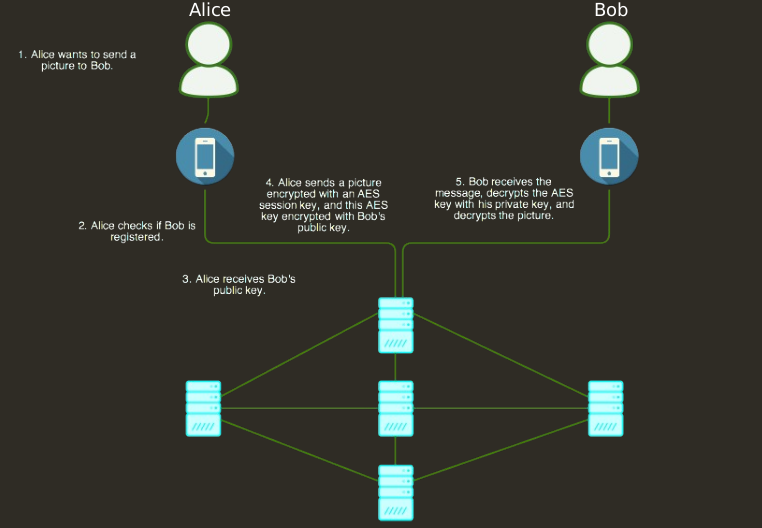
\includegraphics[width=16cm]{images/architecture/architecture}
	\caption{Puzzlr: General Architecture.}
	\label{Figure 1}
      \end{figure}
      \subsection{Registration Phase}
      
	\paragraph{}
	  When two clients want to register on the application, say Alice and Bob, they will both generate an RSA key pair. Their respective public keys are then sent to the server to be stored on the database (figure 2).
	  
	  \begin{figure}[H]  
	    \centering
	    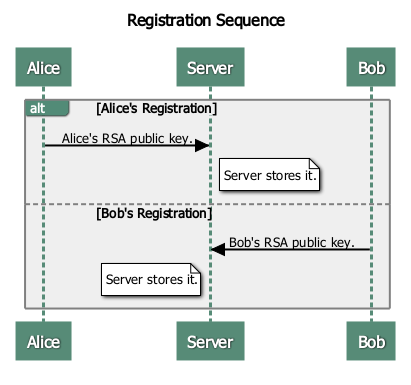
\includegraphics[width=8cm]{images/architecture/registrationsequence}
	    \caption{Registration phase Sequence Diagram.}
	  \end{figure}
	  \subsection{Retrieval of Other Correspondant's Public key}
	  \paragraph{}
	  
	    If let's say Alice wants to send a message to Bob, she will first have to find his corresponding public key. To achieve that, she will send a request to the server which will query the database to check if Alice and Bob are both registered first, if that is the case, the server will then send Bob's public key to Alice (figure 3).
	    
	    \begin{figure}[H]
	      \centering
	      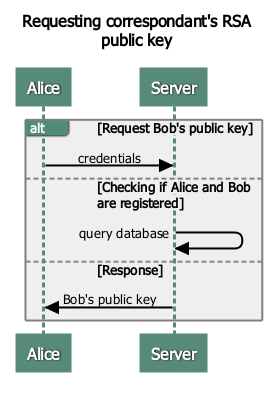
\includegraphics[width=8cm]{images/architecture/requestingcorrespondant'sRSApublickey}
	      \caption{Requesting Correspondant's RSA public key Sequence Diagram.}
	    \end{figure}
	    
	    
	    \subsection{Picture Sending and Receival}
	    \paragraph{}
	    
	    After retrieving Bob's public key from the server, Alice will now do the following steps (figure 4):
	    
	    \begin{itemize}
	     \item Choose a picture to send.
	     \item Generate a session key (AES) and a MAC key.
	     \item Generate a random IV.
	     \item Encrypt the AES key, the MAC key, and her username using Bob's public key (message 1).
	     \item Encrypt the picture that she picked with the AES key and the IV (message 2).
	     \item Generate a MAC tag using the MAC key on the second message (message 2) and the IV (message 3).
	     \item Send the three messages to the server concatenated (message 1 + message 2 + message 3).
	    \end{itemize}
	    
	    \begin{figure}[H]
	    
	      \centering
	      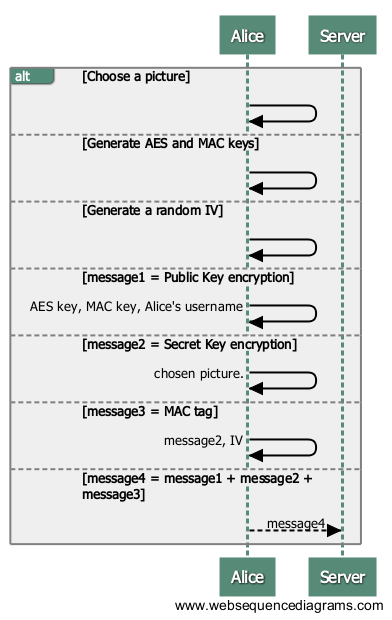
\includegraphics[width=8cm]{images/architecture/picture_sending}
	      \caption{Picture Sending}
	     
	    \end{figure}
	    
	    \paragraph{}
	      On the other hand, when the server receives Alice's message, it will forward this message to Bob. Bob will receive the message and (figure 5):
	      \begin{itemize}
	       \item Recovers the AES key, MAC key, and Alice's username using his private key.
	       \item Checks if the MAC tag received is valid by computing a new one on the received AES ciphertext and the IV, and then compares between them.
	       \item Finally, recovers the picture using the recovered AES key and the IV.
	      \end{itemize}

	    \begin{figure}[H]
	    
	      \centering
	      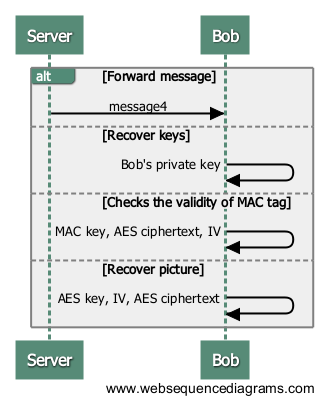
\includegraphics[width=8cm]{images/architecture/receive}
	      \caption{Picture Receival}
	     
	    \end{figure}

	    
	    
	    




	  
      
      
     
      


	
  
\section{Implementations}
  \subsection{Server side}
  \subsection{Client side}
    \subsubsection{Android (Aniss)}
      \paragraph{}
	The Android version is written in Java Programming Language alongside with some parts in XML (the Graphical User Interface). In this project we used Android Studio as an Integrated Developpement Environment (IDE). The application is compatible with almost all versions of Android.
	\paragraph{}
	The source code is open source and is available at this link along with the installation details:
	\paragraph{}
	\color{blue}\underline{https://github.com/aniss05/Puzzlr2}\color{black} 
	  
    \subsubsection{IOS}

\end{document}
